\section{Denotations}\label{sec:denote}

\subsection{Observation Variables}

\begin{figure}
  \centering
  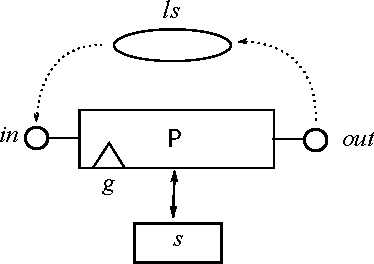
\includegraphics{images/parallel-program}\\
  \caption{High-level view of a concurrent program}
  \label{fig:high-level-prog}
\end{figure}
(See Fig. \ref{fig:high-level-prog}).

A key feature of this UTP semantics is that we have a key distinction
between two groups of observations that we wish to make of a running program.
\begin{description}
  \item[Dynamic State]~\\
    Both the global shared state and control-flow label-set
    are observations that change as the program executes.
    So our UTP theory will need to record both before- and after-values
    for both of these.
    \RLEQNS{
       s, s' &:& State        & \elabel{obs-s}
    \\ ls, ls' &:& \power Lbl & \elabel{obs-ls}
    }
  \item[Static Parameters]~\\
    The labels and generators associated with any given program
    construct are fixed during the lifetime of the program.
    They are determined statically by the context of each construct.
    For this reason we do not distinguish between before- and after-values
    \RLEQNS{
       in, out &:& Lbl & \elabel{obs-in-out}
    \\ g &:& Gen       & \elabel{obs-g}
    }
\end{description}
So our UTP theory has alphabet
\[
  \alpha P  = \setof{s,s',ls,ls',in,out,g}
  \qquad
  \elabel{alpha-P}
\]
and hence is based on a non-homogeneous relation.
This will not turn out to be problematical because
the formulation of the theory as described below will largely isolate the
two classes of observations.



\subsubsection{Ground Expressions}

We assume a general notion of expressions ($e$)
and say that an expression $e$ is ``ground''
if its free variables are limited to only $g$, $in$ and $out$.
We say that a predicate is ground if all constituent expressions
are ground.
\RLEQNS{
   isGnd(e) &\defs&  FV(e) \subseteq \setof{g,in,out}
   & \elabel{gnd-expr-def}
\\ isGnd(P) &\defs&  FV(P) \subseteq \setof{g,in,out}
   & \elabel{gnd-pred-def}
}
This means that ground expressions in this setting can only
define either generators, label-sets, or atomic predicates
over these.
Indeed, generator expressions are ground by construction,
because the only variable they contain is precisely $g$.
It also means that a ground expression can always be simplified
to either a generator expression, enumerated label-set,
and any ground predicate to either true (valid) or false (a contradiction).



\subsection{``Standard'' UTP Predicates}

By ``standard'' UTP predicates,
we mean sequential composition ($\_\seq\_$), skip ($\Skip$),
conditionals $\_\cond\_\_$, and iteration ($\_*\_$).
We put ``standard'' in quotes because we are defining these
in the context of our non-homogeneous alphabet,
which is itself non-standard.

Those familiar with UTP may wonder why we distinguish between
sequential composition in the language ($\cseq$)
and UTP sequential composition ($\seq$).
In UTP theories of sequential programming,
and reactive systems like CSP, sequential composition
in the language has relational predicate composition
as its semantics,
and so the same symbol is used for both.
In concurrent shared-variable programs,
there is no such coincidence between the language operator,
and its semantics.
The precise interpretation of UTP sequential composition ($\seq$)
in this theory will be explained when we introduce the
actual denotational semantics in Section \ref{ssec:UTP-denote}.

Given a non-homogeneous alphabet,
some care has to be taken to define standard notions
from UTP theories, such as sequential composition ($\seq$),
and its unit predicate Skip $\Skip$.
The important thing here turns out to be that these concepts
completely ignore the static parameters.
So the definition of standard sequential composition
defines a mid-point state based solely on $s$ and $ls$:
\RLEQNS{
   P \seq Q
   &\defs& \exists s_m,ls_m \bullet
\\ && \qquad P[s_m,ls_m/s',ls'] \land Q[s_m,ls_m/s,ls]
   & \elabel{UTP-seq-def}
}
Similarly, $\Skip$, the behaviour that immediately terminates
without changing any state, only refers to the dynamic observations:
\RLEQNS{
   \Skip
   &\defs&
   s'= s \land ls'=ls
   & \elabel{UTP-skip-def}
}
It is easy to show that $\Skip$ is both a left- and right-unit for $\seq$,
that $\seq$ is associative,
and that disjunction distributes through it:
\RLEQNS{
   \Skip \seq P &=~P~=& P \seq \Skip & \elabel{seq-unit}
\\ P \seq (Q \seq R) &=& (P \seq Q) \seq R & \elabel{seq-assoc}
\\ P \seq (Q \lor R) &=& P \seq Q \lor P \seq R & \elabel{seq-or-distr}
\\ (P \lor Q) \seq R &=& P \seq R \lor Q \seq R & \elabel{or-seq-distr}
}
Note that we assume that $\seq$ binds more tightly than $\lor$.
We also note the following law, an easy consequence of the above laws:
\RLEQNS{
   (\Skip \lor P) \seq (\Skip \lor Q)
   &=&
   \Skip \lor P \lor Q \lor P\seq Q
   & \elabel{skip-lor-twice}
}
It, and its generalisation will play an important role
in what is to come.
Also important is that ground predicates in conjunction
with a sequential composition can be pushed inside:
\RLEQNS{
   K \land (P \seq Q)
   &=& K \land P \seq Q & \elabel{GND-and-seq-L}
\\ &=& P \seq K \land Q & \elabel{GND-and-seq-R}
\\ &=& K \land P \seq K \land Q & \elabel{GND-and-seq-both}
\\ K \seq K &=& K & \elabel{GND-seq-GND-is-GND}
}
where $isGnd(K)$, and $\land$ binds tighter than $\seq$.


Given the definitions above,
then the definitions of UTP conditionals and iteration
are quite standard.
\RLEQNS{
   P \cond C Q
   &\defs&
   C \land P \lor \lnot C \land Q
   & \elabel{UTP-cond-def}
\\ C * P
   &=&
   P ; C * P \cond C \Skip
   & \elabel{UTP-loop-unroll}
}
For iteration we just present the loop unrolling law, as the most useful here.

We also define a specialised form of sequential composition
to be used when neither component refers to $ls$ or $ls'$,
and its unit $ii$:
\RLEQNS{
   P \seq_s Q
   &\defs&
   \exists s_m \bullet P[s_m/s'] \land Q[s_m/s]
   & \elabel{UTP-s-seq-def}
\\ ii &\defs& s'=s & \elabel{ii-def}
\\ ii \seq_s a \quad=& a &=\quad a \seq_s ii & \elabel{seq-s-unit}
}
Note that if neither predicate mentions $ls$ or $ls'$
then the effect of $\seq$ and $\seq_s$ is the same.
We often omit the $s$ subscript when its use is clear from context.


\subsubsection{Ground Substitutions}

Substitution of expressions for free variables is
an important mechanism used to construct and reason about
UTP theories.
We define a substitution as being ground if the expressions
are all ground, and the target variables belong to $g$, $in$ and $out$.
\RLEQNS{
   isGnd[G,I,O/g,in,out] &\defs& isGnd(G) \land isGnd(I) \land isGnd(O)
   &\elabel{gnd-subs-def}
}
where $G$ is a generator expression,
and $I$ and $O$ are label-set expressions.
In the sequel we shall always assume that $G$, $I$ and $O$
stand for ground expressions, as here.

We shall use $\gamma$ to denote a ground substitution.
\RLEQNS{
  \gamma &=& [G,I,O/g,in,out] &\elabel{gamma-def}
}
The identity substitution can be written as a ground substitution:
\RLEQNS{
  \gamma_{id} &=& [g,in,out/g,in,out] & \elabel{gamma-id-def}
}

The significance of ground substitutions
is that they ignore UTP sequential composition,
in that they distribute through them,
and have no effect on Skip
\RLEQNS{
   (P\seq Q)\gamma &=& P\gamma \seq Q\gamma  & \elabel{seq-gnd-distr}
\\ \Skip\gamma     &=& \Skip                 &\elabel{skip-gamma}
}
They also distribute nicely through our invariant shorthands
\RLEQNS{
   ~\{L_1|\dots|L_n\}\gamma &=& \{L_1\gamma|\dots|L_n\gamma\}
   & \elabel{DL-gamma-subst}
\\ ~[L_1|\dots|L_n]\gamma &=& [L_1\gamma|\dots|L_n\gamma]
   & \elabel{LE-gamma-subst}
}

In addition, the set of all ground substitutions
is closed under substitution composition.
\RLEQNS{
  \exists G,I,O
  &@&
  [G_1,I_1,O_1/g,in,out] [G_2,I_2,O_2/g,in,out]
  =
   [G,I,O/g,in,out]
\\  && \elabel{gnd-sub-closure}
}
We can even give a direct definition of the result:
\RLEQNS{
   [G_1,I_1,O_1/g,in,out]\gamma_2
   &=&
   [G_1\gamma_2,I_1\gamma_2,O_1\gamma_2/g,in,out]
   & \elabel{gnd-sub-comp}
}


\subsubsection{Sound Substitutions}

Unfortunately, there are ground substitutions
that can break the unique label properties
we have worked so hard to achieve with our label generators.
A good example of this is $[g,\ell_g,\ell_g/g,in,out]$,
which can transform an invariant respecting predicate $P$
into one that violates that invariant in a strong way.

A ground substitution $[G,I,O/g,in,out]$ is sound
if the disjoint label invariant $\setof{I|G|O}$ is true.
\RLEQNS{
   isSound[G,I,O/g,in,out] &\defs& \setof{I|G|O}
   & \elabel{sound-sub-def}
}
We shall use $\varsigma$ to denote a sound substitution
\RLEQNS{
   \varsigma &=& [G,I,O/g,in,out] \textbf{ where } \setof{I|G|O} &\elabel{vsigma-def}
}
Note that $\gamma_{id}$ is sound.

All the substitutions explicitly given in the semantic rules below
are sound.
So it is particularly important that soundness is preserved by
substitution composition
\RLEQNS{
   isSound(\varsigma_1)
   \land
   isSound(\varsigma_2)
   &\implies&
   isSound(\varsigma_1\varsigma_2)
   & \elabel{sound-sub-closure}
}




\subsection{Healthiness Conditions}

As is normal in a UTP theory,
we define a number of healthiness conditions
that characterise the predicates we consider to be sound assertions
with respect to our intended interpretation.
At present we have two, called Disjoint Labels
and Wheels-within-Wheels respectively.

\subsubsection{Disjoint Labels}\label{sssec:disj-labels}

We have a general healthiness condition (Disjoint Labels) which asserts that
the labels associated with $in$, $out$ and $g$ are different:
\RLEQNS{
  \lhsDL &\defs& \rhsDL & \elabel{\lblDL}
}
 This is just the Disjoint Labels invariant of
\S\ref{sssec:disjoint-labels}, reformulated as a healthiness condition. Also,
it involves a ground predicate that distributes through sequential composition,
which means the healthiness condition does as well:
\RLEQNS{
  \DL(P\seq Q) &=& \DL(P) \seq \DL(Q) & \eref{DL-seq-distr}
}

\subsubsection{Label Exclusivity}\label{sssec:label-exclude}

We also have a general healthiness condition that strengthens $\DL$ above,
and asserts that at any point in time, the labels $in$ and $out$ are never in
$ls$ together and they are never present if any label from $g$ is:
\RLEQNS{
  \lhsLE &\defs& \rhsLE & \elabel{\lblLE}
}
This is not a ground predicate, and so does not distribute through
sequential composition. However a weaker law does apply:
\RLEQNS{
  \LE(P) \seq \LE(Q)
  &=&
  \LE(P \seq \LE(Q))
  & \elabel{EL-seq}
}
In the sequel we will often use $I$
as shorthand for $[in|g|out]$.



\subsubsection{Wheels-within-Wheels}\label{sssec:WwW}

The key intuition behind this compositional semantics was to take the
$run$ function of the action-system based semantic model used in UTPP,
and drive it inwards to every level of the program.
The original $run$ can be defined in the context of this theory as
\[
  run(P) = ls := \setof{in} ; \lnot (out \in ls) * P
\]
However this failed to keep atomic components ``live''.
They could never be re-executed,
as would be required if they were within an iteration.
Instead it was realised that every construct (atomic and composite)
would have to be within an infinite loop.%
\RLEQNS{
    \true * P &\elabel{WWW-as-loop}
}%
This wrapping of the basic property in an infinite loop
would occur at every level of the program hierarchy,
hence the term ``Wheels within Wheels''.

This bold step turns out to be remarkably effective,
with some quite counter-intuitive outcomes.
However it does depend on a specific tweak to the
definition of an atomic action.
In effect we define an atomic action
as placing a basic action inside such a loop,
but within a non-deterministic choice between it
and a \emph{stuttering} step, denoted by UTP skip:
\RLEQNS{
  \catom a &=& \true * (\Skip \lor A(in|a|out))
}
A result of this is that this stuttering step gets
propagated up to enclosing composites,
so in effect we see $\true * C = \true * (\Skip\lor C)$
where $C$ is any predicate denoting the semantics of a command.
Given that our loop bodies always have such a disjunction,
it then becomes interesting to ask what this looks like:
\RLEQNS{
  \true * (\Skip \lor P) &=& \bigvee_{i \in \Nat} P^i
  & \elabel{loop-as-NDC}
}
We find that such a loop is equivalent to a non-deterministic
choice over the number of times that $P$ is repeated,
including zero.

We choose to \emph{define} the healthiness condition as
this large choice.
\RLEQNS{
   P^0 & \defs& \Skip           & \elabel{seq-0}
\\ P^{i+1} & \defs& P \seq P^i  & \elabel{seq-i-plus-1}
\\ \lhsWWW &\defs& \rhsWWW & \elabel{\lblWWW}
}
 We note explicitly here that, in effect, our semantic model is based on
unbounded non-determinism.

For $\WWW$ to be a proper healthiness condition
is has to be monotonic and idempotent.
\RLEQNS{
   P \refinedby Q &\implies& \WWW(P) \refinedby \WWW(Q)
   & \elabel{WWW-monotonic}
\\ \WWW(\WWW(P)) &=& \WWW(P) & \elabel{WWW-idempotent}
}
The latter is easy to show once we realise that composing the result
of $\WWW(P)$ with itself results in no change:
\RLEQNS{
   \WWW(P) \seq \WWW(P) &=& \WWW(P)  & \elabel{WWW-seq-WWW-is-WWW}
}
Given the definition of $\WWW$, it is easy to see that ground
substitution distributes in:
\RLEQNS{
   \WWW(P)\gamma &=& \WWW(P\gamma) & \elabel{WWW-gnd-subst}
}
as does any top-level conjunction with a ground predicate $K$:
\RLEQNS{
   K \land \WWW(Q) &=& \WWW(K \land Q) & \elabel{WWW-gnd-and-distr}
}



For iteration-free programs
we find that there is a finite $k$ such that $P^k = \false$,
in which case the non-determinism is bounded.
We get these finite results that seem very similar
to the results obtained by using $run$ above.
Using $run$ results in predicates that cannot be composed
to get composite behaviour.
However, using $\WWW$ results in a slight variation,
which is composable!
What turns out to be crucial
to this outcome is the explicit stuttering option.

\subsubsection{WwW Healthiness}

We also note that $\DL$ and $\WWW$ commute,
whereas $\LE$ and $\WWW$ do not:
\RLEQNS{
   \DL(\WWW(P)) &=& \WWW(\DL(P)) & \elabel{DL-WWW-commute}
\\ \LE(\WWW(P))  &=&  I \land \bigvee_{i \in \Nat} P^i
\\ &\neq& & \elabel{LE-WWW-no-commute}
\\ \WWW(\LE(P)) &=& \bigvee_{i \in \Nat} (I \land P)^i
}

With this in mind we define our overall healthiness condition as
\RLEQNS{
   \lhsW &\defs& \rhsW & \elabel{\lblW}
}

\subsection{UTP Denotational Semantics}\label{ssec:UTP-denote}



To proceed we shall first introduce the notation of a Basic Action,
which is the lifting of an atomic shared state transformer $a$
into something that waits for itself to be enabled by appropriate labels.
Then we give the semantics of each language construct in turn.


\subsubsection{Basic Action}\label{sssec:basic-action}

Basic Action $A(E|a|N)$ is enabled when all the labels in $E$ are present in
the global label-set and atomic action $a$ does not evaluate to $\false$ in
the current program state. If so enabled,  it performs action $a$, removes
the labels in $E$ from the label-set, and adds in those in $N$.
\RLEQNS{
   \lhsA &\defs& \rhsA & \elabel{\lblA}
}
 This is a basic building block that is used in subsequent definitions, both
for lifting atomic state change actions, and for defining control-flow label
management.

A key property of basic actions is that ground substitutions
can be driven inside
\RLEQNS{
   A(E|a|N)\gamma &=& A(E\gamma|a|N\gamma)
   & \elabel{A-gamma-subs}
}

The denotational semantic definitions below will have
$\WWW(P)$ as a component,
where $P$ will turn out to be a disjunction of lifted atomic actions,
one of which will be $\Skip$.
\[
  P = \Skip \lor A_1 \lor A_2 \lor A_3 \lor \dots
\]
The effect of this is that $\WWW(P)$ itself
will be a disjunction of elements that are
either $\Skip$, one of those actions making up $P$
or the sequential composition, using $\seq$,
of a sequence of two or more of those actions.
\RLEQNS{
   \WWW(P) &=& \bigvee_{i \in \Nat} P^i
\\ &=& \Skip \lor A_1 \lor A_2 \lor A_3 \lor \dots
\\ &\lor& A_1^2 \lor A_2^2 \lor A_3^2 \lor \dots
\\ &\lor& A_1\seq A_2 \lor A_2 \seq A_1 \lor \dots
\\ &\lor& \dots \lor A_3\seq A_3\seq A_1 \seq A_2 \lor \dots
}
In practise, many of these sequential compositions will reduce to $\false$,
because they are not viable---this is discussed in more detail in the section
on calculating with the theory (\S\ref{sec:calc}).

Given a composition $A_3\seq A_3\seq A_1 \seq A_2$ (say),
it is to be interpreted as an observation
of the execution of its components in order,
without any interference from outside.
In effect these terms correspond to mumblings in the denotational
semantics of Brookes\cite{DBLP:journals/iandc/Brookes96}.
So, in this theory,
UTP sequential composition ($\seq$)
 can be thought of as \emph{mumbling composition}.
In a similar vein, the $\Skip$ predicate represents
all the possible stuttering steps in Brookes' semantics.


\newpage
\subsubsection{Atomic Action}

\begin{figure}[h]
  \centering
  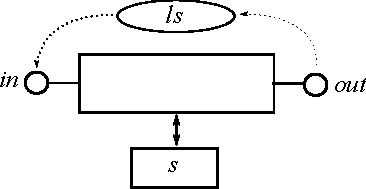
\includegraphics{images/atomic-action}\\
  \caption{Atomic Action}
  \label{fig:atomic-action}
\end{figure}

An atomic action (Fig.\ref{fig:atomic-action})
is a basic action where the enabling label-set is
simply $\setof{in}$, and the new label introduced once complete
is $\setof{out}$.
It has no subcomponents, so it does not use the label generator $g$.

The key invariant here is that $in$ and $out$ are never simultaneously in
$ls$. So we simply wrap the corresponding action with the healthiness
conditions and conjoin our invariant:
\RLEQNS{
  \lhsCA &\defs& \rhsCA & \elabel{\lblCA}
}
 Note here that we write $x$ rather than $\setof{x}$, as a shorthand. This
is why the notation for $A$ uses vertical bars to separate arguments.

We need to show that $A(in|a|out)$ preserves the $\LE$
invariant, under any arbitrary sound substitution $\varsigma$:
\RLEQNS{
   \{in|g|out\}\varsigma
   \land I\varsigma
   \land A(in|a|out)\varsigma &\implies& I'\varsigma
   & \eref{atom-inv-ok}
}
Here $I'$ is simply $I$ with $ls$ replaced by $ls'$.

\subsubsection{Guarded Atomic Action}
In effect there is no real difference between $c \pgrd a$
and $\true \pgrd (c \land a)$,
so in fact we don't need guarded actions as basic.
This is an advantage of treating the atomic action as a relational predicate
on state.

\RLEQNS{
 c \pgrd a &\defs& \catom{c \land a}  &\elabel{sem:pgrd}
}

\subsubsection{Skip}

Skip in the programming language ($\cskip$)
is simply an atomic action that leaves the program state $s$ unchanged:
\RLEQNS{
   \cskip &\defs& \catom{s'=s}  &\elabel{sem:skip}
\\ &=& \catom{ii}
}

%\newpage
\subsubsection{Sequential Composition}

\begin{figure}[h]
  \centering
  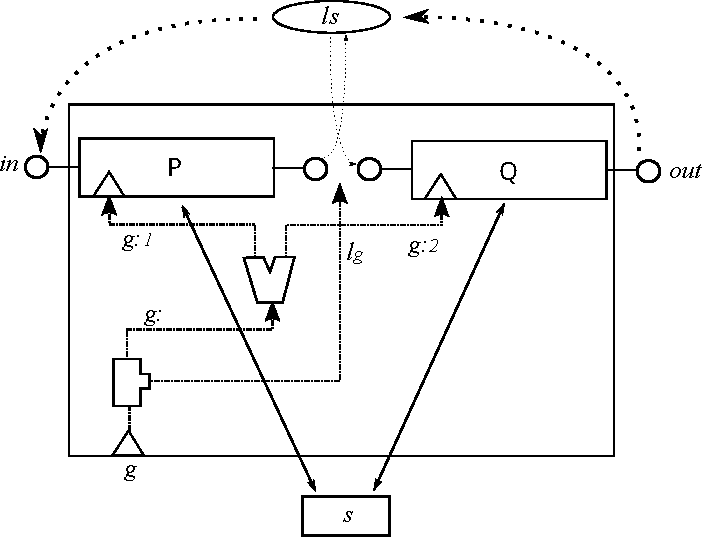
\includegraphics[scale=0.85]{images/seq-comp-actual}
  \caption{Sequential Composition}
  \label{fig:seq-comp}
\end{figure}

In order to sequentially compose $P$ and $Q$ (Fig.\ref{fig:seq-comp}),
we want to arrange for the $out$ label of $P$
to coincide with the $in$ label of $Q$.
We do this by generating a new unique label with our generator $g$,
giving us label $\ell_g$ and the ``leftover'' generator $\g{:}$.
That $\ell_g$ is not the same as either $in$ or $out$
is guaranteed by the $\DL$ invariant.
When then replace all references in $P$ to $out$,
and in $Q$ to $in$, by $\ell_g$.
We also need to ensure that the generators used by $P$ and $Q$
do not produce labels that clash with $in$, $out$, $\ell_g$,
or each others' generator.
We do this by splitting our leftover generator into two parts,
$\g{:1}$ and $\g{:2}$,
and replacing all references to $g$ in both $P$ and $Q$
with these split generators.

So $P$ becomes $P[\g{:1},\ell_g/g,out]$,
and $Q$ is changed to $Q[\g{:2},\ell_g/g,in]$, both substitutions being sound.
Next, we connect our modified $P$ and $Q$ with \emph{disjunction},
and healthify.
\RLEQNS{
   \lhsSEQ &\defs& \rhsSEQ & \elabel{\lblSEQ}
}
For all of this to work we require an invariant
to ensure that only one of $in$, $\ell_g$ or $out$
are ever present in $ls$.
However $\LE$ ensures this as $[in|g|out]$ implies $[in|\ell_g|out]$.
If $A$ actions inside $P$ and $Q$ preserve the invariant,
then so does their composition.
This is immediate by the sound substitution independence
of invariant preservation (c.f., \eref{atom-inv-ok}).



\newpage
\subsubsection{Parallel Composition}

\begin{figure}[h]
  \centering
  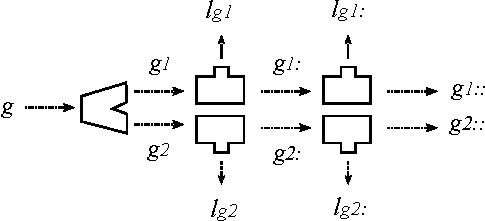
\includegraphics{images/parallel-label-gen}\\
  \caption{Generating labels for Parallel Composition}
  \label{fig:par-lbl-gen}
\end{figure}
Parallel composition $P\parallel Q$ may seem straightforward:
simply leave $in$ and $out$ alone, split $g$ and feed the
two generators into $P$ and $Q$, put into disjunction with each other.
However this won't work. Both $P$ and $Q$ will
have an atomic action enabled by $in$,
and one of these will be non-deterministically chosen to run first.
When it does it will remove $in$ from $ls$,
effectively disabling the other action.
Instead we need to replace the $in$s and $out$s of $P$ and $Q$
with four different labels, using a scheme such as that described
in Fig.\ref{fig:par-lbl-gen}.

We then introduce two new control-flow actions:
the first (Split) is enabled by $in$, and adds into $ls$
the labels replacing the $in$s;
the second (Merge) is enabled by both of the labels replacing the $out$s,
and adds $out$ into $ls$.
In effect, Split enforces that both $P$ and $Q$ start together,
once $P \parallel Q$ has started,
while Merge ensures that $P \parallel Q$ only terminates
when both $P$ and $Q$ have (See Fig.\ref{fig:par-comp}).
\begin{figure}
  \centering
  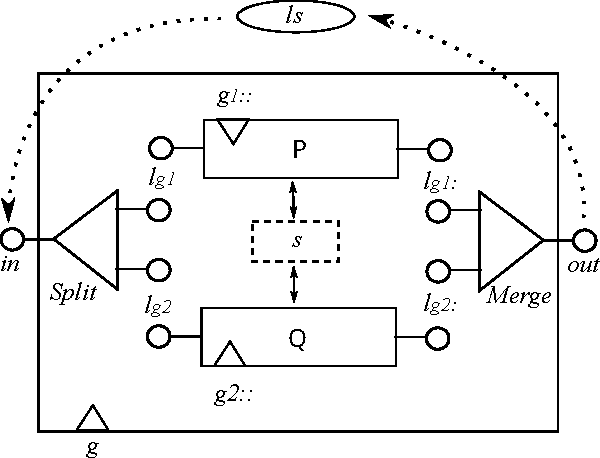
\includegraphics{images/par-comp-actual}
  \caption{Parallel Composition}
  \label{fig:par-comp}
\end{figure}

Putting all of this together gives the following definition
\RLEQNS{
   \lhsPAR
   &\defs&
   \leftW \rhsaPAR \lor {}
   & \elabel\lblPAR
\\&& \phW \rhsbPAR \lor {}
\\&& \phW \rhscPAR \lor {}
\\&& \phW \rhsdPAR \rghtW
}
The behaviour for parallel has not only to ensure
that $in$ and $out$ are never in $ls$ together
or when any of the four generated labels are,
but also that the labels that replace $in$
are never in $ls$ at the same time as the corresponding
replacements for $out$ (see also \S\ref{sssec:label-exclusivity}).
The first part is guaranteed by $\LE$ at this level.
For the second part we note that  the components $P$ and $Q$
both have the $\LE$ invariant, which under the relevant sound substitutions
become $[\ell_{g1}|\g{1::}|\ell_{g1:}]$
and $[\ell_{g2}|\g{2::}|\ell_{g2:}]$ respectively.
This is enough to enforce the correct behaviour of the generated labels.


We need to demonstrate that the Split and Merge actions
preserve the $\LE$ invariant:
\RLEQNS{
   \{in|g|out\}\varsigma
   \land I\varsigma
   && \eref{split-inv-ok}
\\ {} \land [g_{1::}|\ell_{g1}|\ell_{g1:}]\varsigma
\\ {} \land [g_{2::}|\ell_{g2}|\ell_{g2:}]\varsigma
\\ {} \land A(in|ii|\ell_{g1},\ell_{g2})\varsigma
   &\implies&
   I'\varsigma
\\&& {} \land [g_{1::}|\ell_{g1}|\ell_{g1:}]'\varsigma
\\&& {} \land [g_{2::}|\ell_{g2}|\ell_{g2:}]'\varsigma
\\
\\ \{in|g|out\}\varsigma
   \land I\varsigma
   && \eref{merge-inv-ok}
\\ {} \land [g_{1::}|\ell_{g1}|\ell_{g1:}]\varsigma
\\ {} \land [g_{2::}|\ell_{g2}|\ell_{g2:}]\varsigma
\\ {} \land A(|\ell_{g1:},\ell_{g2:}|ii|out)\varsigma
   &\implies&
   I'\varsigma
\\&& {} \land [g_{1::}|\ell_{g1}|\ell_{g1:}]'\varsigma
\\&& {} \land [g_{2::}|\ell_{g2}|\ell_{g2:}]'\varsigma
}


\newpage
\subsubsection{Nondeterministic Choice}

\begin{figure}[h]
  \centering
  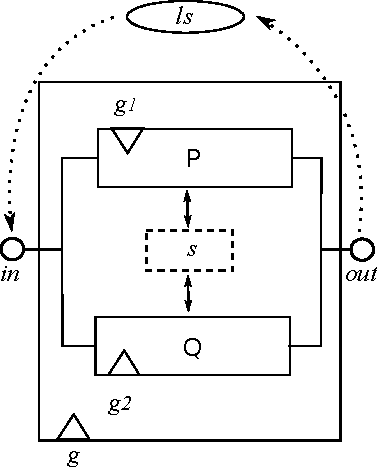
\includegraphics{images/nondet-actual}
  \caption{Nondeterministic Choice}
  \label{fig:nondet-choice}
\end{figure}

Nondeterministic choice $P+Q$ is very simple:
we simply split the generator and pass one part
into each component. We do not need to relabel $in$
or $out$.
The first atomic action enabled by $in$ to
run in either component will disable all other such actions in both components,
because it will remove $in$ from the label-set.
However we do need to extend the $\LE$ invariant a little,
to assert that labels from one side are never present when labels from
the other side are.
\RLEQNS{
   \lhsNDC &\defs& \invNDC \land \rhsNDC & \elabel{\lblNDC}
}


$\LE$ invariant preservation --- if an action in $P$ is enabled,
and the invariant holds, then no labels from $Q$ are present.
$P$ can only modify $ls$ membership for labels in $\g1$,
so it cannot invalidate the invariant by mixing in labels from $\g2$.
(And vice-versa).


\newpage
\subsubsection{Nondeterministic Loop}

\begin{figure}[h]
  \centering
  % Requires \usepackage{graphicx}
  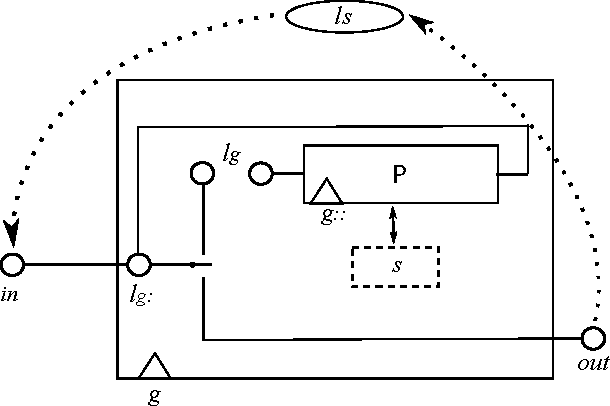
\includegraphics{images/kleene-star-actual}
  \caption{Nondeterministic Loop}
  \label{fig:nondet-loop}
\end{figure}

A nondeterministic loop $P^*$  starts with a non-deterministic choice
regarding if it will immediately terminate,
or perform an iteration.
In the former case we go directly to $out$,
while in the latter we need a new label ($\ell_g$)
which replaces the $in$ of $P$.
We also need to ``buffer'' $in$, by not using it as the terminate/continue
decision point. Instead we use yet another label ($\ell_{g:}$
as the one in $ls$ when deciding if to stop of continue.
When $P$ terminates, we immediately go back to the decision point $\ell_{g:}$
to choose again.
\RLEQNS{
   \lhsSTAR
   &\defs&
   \leftW \rhsaSTAR \lor {}
   & \elabel\lblSTAR
\\&& \phW \rhsbSTAR \lor {}
\\&& \phW \rhscSTAR \lor {}
\\&& \phW \rhsdSTAR \rghtW
}
To understand why we cannot use $in$ itself as the decision point,
consider the program $P^*+Q^*$. If the decision point is $in$
then every time either $P$ or $Q$ finish an execution,
both become enabled. This is because $+$ does not re-label $in$.
Another possibility would be to have $+$ have actions to make
a choice between the two sides, and then this loop could
use $in$ as a decision point.
But then this breaks a property that $P$ never puts $in$ into $ls$,
but only removes it.

$\LE$ invariant preservation
\RLEQNS{
   \{in|g|out\}\varsigma
   \land [in|\ell_{g1}|out]\varsigma
   && \eref{ndc-exit-inv-ok}
\\ {} \land A(in|ii|out)\varsigma
   &\implies&
   [in|\ell_{g1}|out]'\varsigma
\\ \{in|g|out\}\varsigma
   \land [in|\ell_{g1}|out]\varsigma
   && \eref{ndc-loop-inv-ok}
\\ {} \land A(in|ii|\ell_{g1})\varsigma
   &\implies&
   [in|\ell_{g1}|out]'\varsigma
}


\newpage
\subsubsection{Conditional Choice}

\begin{figure}[h]
  \centering
  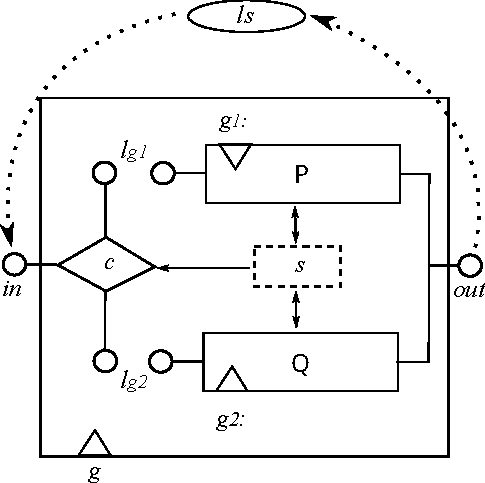
\includegraphics{images/conditional-actual}
  \caption{Conditional Choice}
  \label{fig:conditional}
\end{figure}


The semantics for conditional choice $P \dcond c Q$
is different to that for non-deterministic choice.
The difference is that we need two control-flow actions
have the condition $c$, or its negation as appropriate,
conjoined with the underlying program state skip action $ii$.
This ensures that the control-flow action is only able to proceed
if $in$ is in $ls$ and the condition or its negation is true
in the current state $s$.
\RLEQNS{
   \lhsCND
   &\defs&
   \leftW \rhsaCND \lor {}
   & \elabel\lblCND
\\&& \phW \rhsbCND \lor {}
\\&& \phW \rhscCND \lor {}
\\&& \phW \rhsdCND \rghtW
\\&& {} \land \invCND
}
We do need to extend the $\LE$ invariant to ensure
that once one side or other of the conditional is active,
the other remains inactive.


$\LE$ invariant preservation
\RLEQNS{
   \{in|g|out\}\varsigma
   \land [in|\ell_{g1}|\ell_{g2}|out]\varsigma
   && \eref{cond-1-inv-ok}
\\ {} \land A(in|c \land ii|\ell_{g1})\varsigma
   &\implies&
   [in|\ell_{g1}|\ell_{g2}|out]'\varsigma
\\ \{in|g|out\}\varsigma
   \land [in|\ell_{g1}|\ell_{g2}|out]\varsigma
   && \eref{cond-2-inv-ok}
\\ {} \land A(in|\lnot c \land ii|\ell_{g2})\varsigma
   &\implies&
   [in|\ell_{g1}|\ell_{g2}|out]'\varsigma
}

\newpage
\subsubsection{Conditional Loop}

\begin{figure}[h]
  \centering
  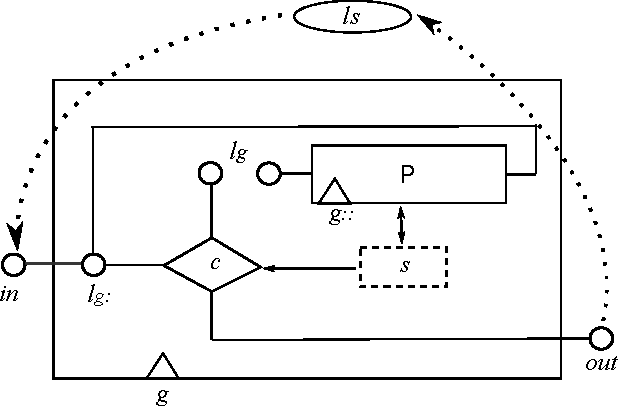
\includegraphics{images/iteration-actual}
  \caption{Conditional Loop}
  \label{fig:cond-loop}
\end{figure}

See the previous section about conditional choice regarding the
role of state-condition $c$---the same idea applies here too.
\RLEQNS{
   \lhsITER
   &\defs&
   \leftW \rhsaITER \lor {}
   & \elabel\lblITER
\\&& \phW \rhsbITER \lor {}
\\&& \phW \rhscITER \lor {}
\\&& \phW \rhsdITER \rghtW
}


$\LE$ invariant preservation
\RLEQNS{
   \{in|g|out\}\varsigma
   \land [in|\ell_{g1}|out]\varsigma
   && \eref{cond-exit-inv-ok}
\\ {} \land A(in|\lnot c \land ii|out)\varsigma
   &\implies&
   [in|\ell_{g1}|out]'\varsigma
\\ \{in|g|out\}\varsigma
   \land [in|\ell_{g1}|out]\varsigma
   && \eref{cond-loop-inv-ok}
\\ {} \land A(in|c \land ii|\ell_{g1})\varsigma
   &\implies&
   [in|\ell_{g1}|out]'\varsigma
}

\subsection{Semantics Summary}\label{ssec:sem-recap}


\RLEQNS{
   \lhsDL &\defs& \rhsDL & \eref{\lblDL}
\\
\\ \lhsLE &\defs& \rhsLE & \eref{\lblLE}
\\
\\ P^0 & \defs& \Skip           & \eref{seq-0}
\\ P^{i+1} & \defs& P \seq P^i  & \eref{seq-i-plus-1}
\\
\\ \lhsWWW &\defs& \rhsWWW & \eref{\lblWWW}
\\
\\ \lhsW &\defs& \rhsW & \eref{\lblW}
\\
\\ \lhsA &\defs& \rhsA & \eref{\lblA}
\\
\\ \lhsCA &\defs& \rhsCA & \eref{\lblCA}
\\
\\ \lhsSEQ &\defs& \rhsSEQ & \eref{\lblSEQ}
\\
\\ \lhsPAR
   &\defs&
   \leftW \rhsaPAR \lor {}
   & \eref\lblPAR
\\&& \phW \rhsbPAR \lor {}
\\&& \phW \rhscPAR \lor {}
\\&& \phW \rhsdPAR \rghtW
\\
\\ \lhsNDC &\defs& \invNDC \land \rhsNDC & \eref{\lblNDC}
\\
\\ \lhsSTAR
   &\defs&
   \leftW \rhsaSTAR \lor {}
   & \eref\lblSTAR
\\&& \phW \rhsbSTAR \lor {}
\\&& \phW \rhscSTAR \lor {}
\\&& \phW \rhsdSTAR \rghtW
\\
\\ \lhsCND
   &\defs&
   \leftW \rhsaCND \lor {}
   & \eref\lblCND
\\&& \phW \rhsbCND \lor {}
\\&& \phW \rhscCND \lor {}
\\&& \phW \rhsdCND \rghtW
\\&& {} \land \invCND
\\
\\ \lhsITER
   &\defs&
   \leftW \rhsaITER \lor {}
   & \eref\lblITER
\\&& \phW \rhsbITER \lor {}
\\&& \phW \rhscITER \lor {}
\\&& \phW \rhsdITER \rghtW
}


\newpage
\subsection{Key Semantic Properties}

\begin{description}
  \item[Label Movement]
    We need to show that in any construct,
    no basic action is enabled by $out$
    and that it is only added into $ls$.
    A complementary property holds for $in$,
    which is only removed from $ls$.
    These properties hold under any sound substitution $\varsigma$ as well.
\end{description}
